\documentclass[11pt,a4paper]{article}
\usepackage[margin=1in]{geometry}
\usepackage{booktabs}
\usepackage{xcolor}
\usepackage{colortbl}
\usepackage{graphicx}
\usepackage{pgfplots}
\usepackage{pgfplotstable}
\usepackage{tikz}
\usepackage{hyperref}
\usepackage{float}
\usetikzlibrary{positioning, arrows.meta, shapes.geometric, calc}
\pgfplotsset{compat=1.18}

% Color definitions
\definecolor{keepgreen}{HTML}{2ECC71}
\definecolor{rejectred}{HTML}{E74C3C}
\definecolor{investyellow}{HTML}{F39C12}
\definecolor{highblue}{HTML}{2980B9}
\definecolor{medskyblue}{HTML}{5DADE2}
\definecolor{lowgray}{HTML}{95A5A6}
\definecolor{deadblack}{HTML}{2C3E50}

\title{Research Ideation Swarm: Visual Synthesis\\
\large 120-Round Multi-Agent Discovery System for QCML Geometric Observatory}
\author{QCML Research Team}
\date{March 8, 2026}

\begin{document}
\maketitle

\section{Overview}

120 research questions explored across 11 themes using hierarchical agent swarm (Agent~0 $\to$ Knights $\to$ Workers). Smoke test protocol: 4 crises (GFC, COVID, 2022, SVB), keep threshold $d > 0.3$.

\begin{center}
\Large\textbf{82 Keep \quad 29 Reject \quad 9 Investigate}
\end{center}

%% ===== SECTION 1: Theme Breakdown =====
\section{Verdict Distribution by Theme}

\begin{figure}[H]
\centering
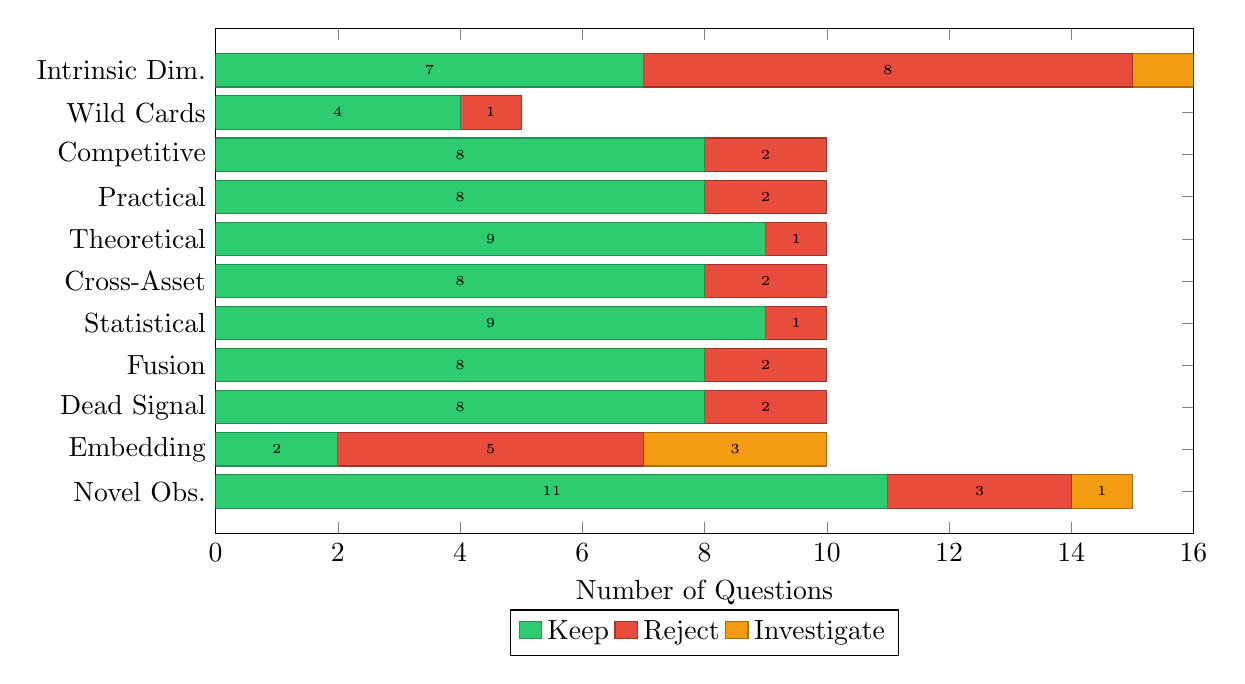
\begin{tikzpicture}
\begin{axis}[
    xbar stacked,
    width=14cm, height=8cm,
    xlabel={Number of Questions},
    symbolic y coords={
        Intrinsic Dim.,
        Wild Cards,
        Competitive,
        Practical,
        Theoretical,
        Cross-Asset,
        Statistical,
        Fusion,
        Dead Signal,
        Embedding,
        Novel Obs.
    },
    ytick=data,
    y dir=reverse,
    legend style={at={(0.5,-0.15)}, anchor=north, legend columns=3},
    bar width=12pt,
    xmin=0, xmax=16,
    nodes near coords,
    every node near coord/.append style={font=\tiny},
]
\addplot[fill=keepgreen, draw=keepgreen!70!black] coordinates {
    (11,Novel Obs.) (2,Embedding) (8,Dead Signal) (8,Fusion)
    (9,Statistical) (8,Cross-Asset) (9,Theoretical) (8,Practical)
    (8,Competitive) (4,Wild Cards) (7,Intrinsic Dim.)
};
\addplot[fill=rejectred, draw=rejectred!70!black] coordinates {
    (3,Novel Obs.) (5,Embedding) (2,Dead Signal) (2,Fusion)
    (1,Statistical) (2,Cross-Asset) (1,Theoretical) (2,Practical)
    (2,Competitive) (1,Wild Cards) (8,Intrinsic Dim.)
};
\addplot[fill=investyellow, draw=investyellow!70!black] coordinates {
    (1,Novel Obs.) (3,Embedding) (0,Dead Signal) (0,Fusion)
    (0,Statistical) (0,Cross-Asset) (0,Theoretical) (0,Practical)
    (0,Competitive) (0,Wild Cards) (5,Intrinsic Dim.)
};
\legend{Keep, Reject, Investigate}
\end{axis}
\end{tikzpicture}
\caption{Verdict distribution across 11 research themes. Intrinsic Dimension has the lowest keep rate (35\%), while Statistical and Theoretical have the highest (90\%).}
\end{figure}

%% ===== SECTION 2: Effect Size Heatmap =====
\section{Effect Size Table: Questions with Empirical Results}

\begin{table}[H]
\centering
\small
\caption{All questions with measured Cohen's $d$, sorted by effect size. Colors: \colorbox{keepgreen!30}{keep}, \colorbox{rejectred!30}{reject}.}
\begin{tabular}{@{}rlccl@{}}
\toprule
\textbf{Rank} & \textbf{ID} & \textbf{$d$} & \textbf{Status} & \textbf{Question (abbreviated)} \\
\midrule
1  & Q33 & 2.018 & \cellcolor{keepgreen!30}keep & LSTM + attention resurrection \\
2  & Q45 & 1.775 & \cellcolor{keepgreen!30}keep & HClust fusion \\
3  & Q30 & 1.690 & \cellcolor{keepgreen!30}keep & Top-3 curated ensemble \\
4  & Q93 & 1.631 & \cellcolor{keepgreen!30}keep & VIX benchmark \\
5  & Q107 & 1.411 & \cellcolor{keepgreen!30}keep & Ground state energy $E_0(x)$ \\
6  & Q63 & 1.375 & \cellcolor{keepgreen!30}keep & Multi-market embedding \\
7  & Q65 & 1.366 & \cellcolor{keepgreen!30}keep & Market breadth embedding \\
8  & Q92 & 1.329 & \cellcolor{keepgreen!30}keep & Turbulence index comparison \\
9  & Q16 & 1.327 & \cellcolor{keepgreen!30}keep & Hilbert dim=16 \\
10 & Q42 & 1.260 & \cellcolor{keepgreen!30}keep & Switching model \\
11 & Q41 & 1.258 & \cellcolor{rejectred!30}reject & Stacking/GBM (overfits) \\
12 & Q102 & 1.175 & \cellcolor{keepgreen!30}keep & Spectral gap ratio \\
13 & Q24 & 1.144 & \cellcolor{keepgreen!30}keep & Soft normalization \\
14 & Q02 & 1.121 & \cellcolor{keepgreen!30}keep & OTOC detector \\
15 & Q44 & 1.009 & \cellcolor{keepgreen!30}keep & MI-weighted fusion \\
16 & Q90 & 0.962 & \cellcolor{keepgreen!30}keep & Absorption ratio \\
17 & Q31 & 0.898 & \cellcolor{keepgreen!30}keep & BOCPD short hazard \\
18 & Q01 & 0.849 & \cellcolor{keepgreen!30}keep & Loschmidt echo \\
19 & Q39 & 0.842 & \cellcolor{keepgreen!30}keep & Hedge/MW fusion \\
20 & Q64 & 0.816 & \cellcolor{keepgreen!30}keep & Regional contagion \\
21 & Q10 & 0.791 & \cellcolor{keepgreen!30}keep & Wasserstein distance \\
22 & Q32 & 0.763 & \cellcolor{keepgreen!30}keep & Transfer entropy fix \\
23 & Q36 & 0.762 & \cellcolor{rejectred!30}reject & Attention fusion \\
24 & Q35 & 0.762 & \cellcolor{keepgreen!30}keep & Spectral flow L1 \\
25 & Q38 & 0.739 & \cellcolor{keepgreen!30}keep & Copula fusion \\
26 & Q04 & 0.696 & \cellcolor{keepgreen!30}invest. & Entanglement entropy \\
27 & Q101 & 0.633 & \cellcolor{keepgreen!30}keep & Intrinsic dimension (QCML) \\
28 & Q40 & 0.693 & \cellcolor{keepgreen!30}keep & BMA fusion \\
29 & Q29 & 0.692 & \cellcolor{keepgreen!30}keep & Geom.\ consensus OR \\
30 & Q34 & 0.669 & \cellcolor{keepgreen!30}keep & Kernel PCA tuned \\
31 & Q09 & 0.656 & \cellcolor{keepgreen!30}keep & Persistent homology \\
32 & Q91 & 0.656 & \cellcolor{keepgreen!30}keep & TDA comparison \\
33 & Q11 & 0.652 & \cellcolor{keepgreen!30}keep & Thouless energy \\
34 & Q13 & 0.651 & \cellcolor{keepgreen!30}keep & Modular Hamiltonian \\
35 & Q89 & 0.637 & \cellcolor{keepgreen!30}keep & Hurst exponent \\
36 & Q43 & 0.633 & \cellcolor{keepgreen!30}keep & Rank aggregation \\
37 & Q56 & 0.619 & \cellcolor{keepgreen!30}keep & Bond markets \\
38 & Q14 & 0.594 & \cellcolor{rejectred!30}reject & Quantum discord \\
39 & Q08 & 0.541 & \cellcolor{keepgreen!30}keep & Husimi Q-function \\
40 & Q58 & 0.540 & \cellcolor{keepgreen!30}keep & Commodity markets \\
41 & Q28 & 0.539 & \cellcolor{keepgreen!30}keep & Curvature rate fix \\
42 & Q07 & 0.537 & \cellcolor{keepgreen!30}keep & Partition function \\
43 & Q37 & 0.525 & \cellcolor{keepgreen!30}keep & Majority vote \\
44 & Q06 & 0.443 & \cellcolor{keepgreen!30}keep & Kibble-Zurek \\
45 & Q104 & 0.422 & \cellcolor{keepgreen!30}keep & Effective dimension (PR) \\
46 & Q15 & 0.431 & \cellcolor{keepgreen!30}keep & Floquet analysis \\
47 & Q22 & 0.398 & \cellcolor{rejectred!30}reject & Multi-scale embedding \\
48 & Q57 & 0.387 & \cellcolor{keepgreen!30}keep & Crypto markets \\
49 & Q17 & 0.367 & \cellcolor{keepgreen!30}invest. & Neural embedding \\
50 & Q79 & 0.320 & \cellcolor{keepgreen!30}keep & Reduced cost (dim=8) \\
51 & Q12 & 0.301 & \cellcolor{keepgreen!30}keep & Zak phase \\
52 & Q60 & 0.282 & \cellcolor{keepgreen!30}keep & FX markets \\
53 & Q103 & 0.269 & \cellcolor{rejectred!30}reject & Dimension rate $\Delta d/\Delta t$ \\
54 & Q62 & 0.267 & \cellcolor{rejectred!30}reject & VIX term structure \\
55 & Q05 & 0.228 & \cellcolor{rejectred!30}reject & QGT off-diagonal \\
56 & Q03 & 0.216 & \cellcolor{rejectred!30}reject & Chern number \\
57 & Q18 & 0.149 & \cellcolor{rejectred!30}reject & Takens embedding \\
58 & Q26 & 0.028 & \cellcolor{rejectred!30}reject & QGT phase rigidity \\
59 & Q27 & 0.013 & \cellcolor{rejectred!30}reject & Berry velocity coupling \\
\bottomrule
\end{tabular}
\end{table}

%% ===== SECTION 3: Network of Interconnections =====
\section{Question Interconnection Network}

\begin{figure}[H]
\centering
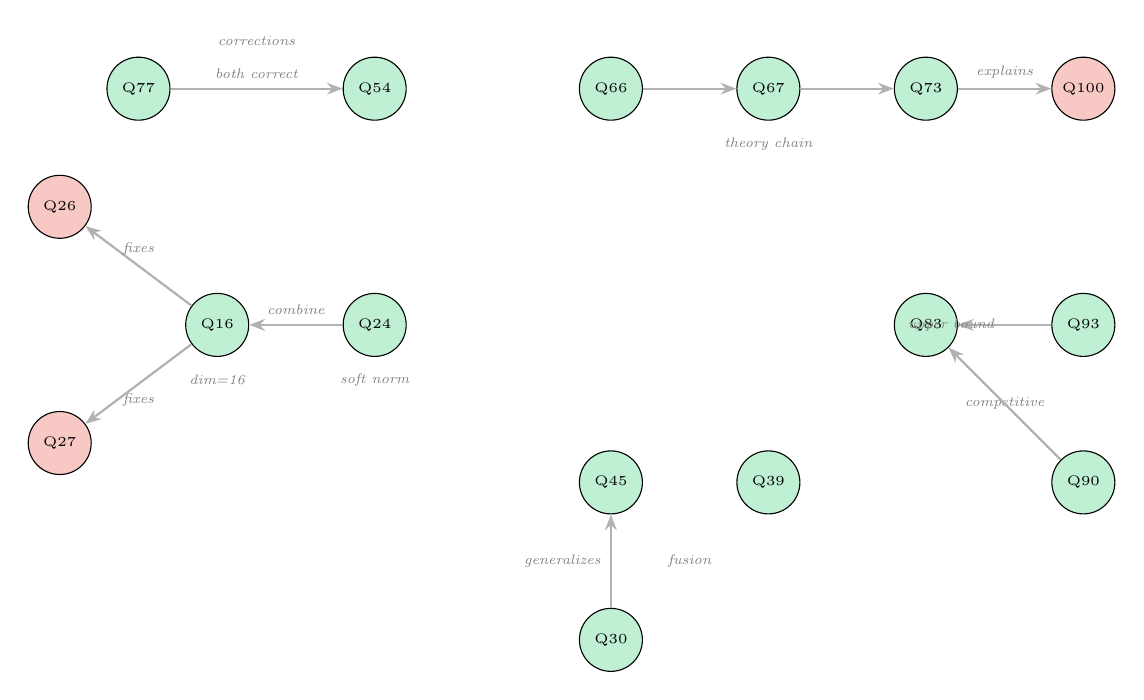
\begin{tikzpicture}[
    node distance=2cm,
    qnode/.style={circle, draw, minimum size=0.8cm, font=\tiny, inner sep=1pt},
    keepnode/.style={qnode, fill=keepgreen!30},
    rejectnode/.style={qnode, fill=rejectred!30},
    edge/.style={-{Stealth[length=2mm]}, thick, gray!60},
    label/.style={font=\tiny\itshape, text=gray}
]

% Central cluster: Embedding improvements
\node[keepnode] (q16) at (0,0) {Q16};
\node[label] at (0,-0.7) {dim=16};
\node[keepnode] (q24) at (2,0) {Q24};
\node[label] at (2,-0.7) {soft norm};

% Dead signals connected to Q16
\node[rejectnode] (q26) at (-2,1.5) {Q26};
\node[rejectnode] (q27) at (-2,-1.5) {Q27};

% Theory cluster
\node[keepnode] (q66) at (5,3) {Q66};
\node[keepnode] (q67) at (7,3) {Q67};
\node[keepnode] (q73) at (9,3) {Q73};
\node[rejectnode] (q100) at (11,3) {Q100};
\node[label] at (7,2.3) {theory chain};

% Fusion cluster
\node[keepnode] (q45) at (5,-2) {Q45};
\node[keepnode] (q39) at (7,-2) {Q39};
\node[keepnode] (q30) at (5,-4) {Q30};
\node[label] at (6,-3) {fusion};

% Competitive cluster
\node[keepnode] (q93) at (11,0) {Q93};
\node[keepnode] (q90) at (11,-2) {Q90};
\node[keepnode] (q83) at (9,0) {Q83};
\node[label] at (10,-1) {competitive};

% Corrections
\node[keepnode] (q77) at (-1,3) {Q77};
\node[keepnode] (q54) at (2,3) {Q54};
\node[label] at (0.5,3.6) {corrections};

% Edges
\draw[edge] (q16) -- (q26) node[midway,above,label] {fixes};
\draw[edge] (q16) -- (q27) node[midway,below,label] {fixes};
\draw[edge] (q66) -- (q67);
\draw[edge] (q67) -- (q73);
\draw[edge] (q73) -- (q100) node[midway,above,label] {explains};
\draw[edge] (q90) -- (q83);
\draw[edge] (q93) -- (q83) node[midway,left,label] {upper bound};
\draw[edge] (q30) -- (q45) node[midway,left,label] {generalizes};
\draw[edge] (q24) -- (q16) node[midway,above,label] {combine};
\draw[edge] (q77) -- (q54) node[midway,above,label] {both correct};

\end{tikzpicture}
\caption{Key interconnections between findings. Green = keep, red = reject. Arrows show logical dependencies and explanatory relationships.}
\end{figure}

%% ===== SECTION 4: Dead Signal Resurrection =====
\section{Dead Signal Resurrection Results}

\begin{figure}[H]
\centering
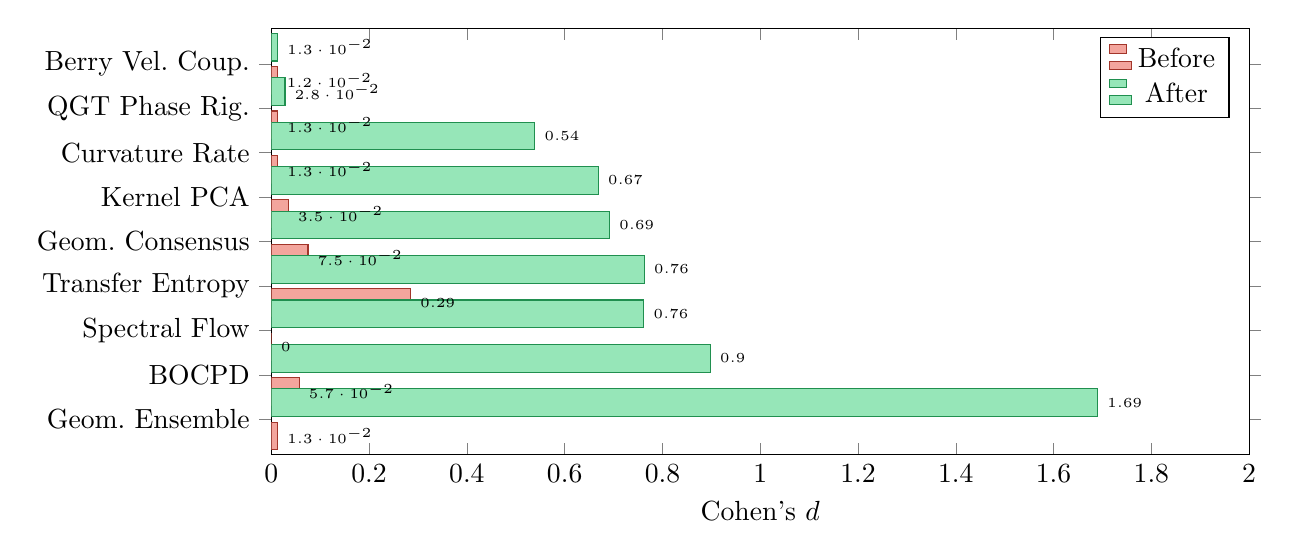
\begin{tikzpicture}
\begin{axis}[
    xbar,
    width=14cm, height=7cm,
    xlabel={Cohen's $d$},
    symbolic y coords={
        Berry Vel.\ Coup.,
        QGT Phase Rig.,
        Curvature Rate,
        Kernel PCA,
        Geom.\ Consensus,
        Transfer Entropy,
        Spectral Flow,
        BOCPD,
        Geom.\ Ensemble
    },
    ytick=data,
    y dir=reverse,
    xmin=0, xmax=2,
    bar width=10pt,
    legend style={at={(0.98,0.98)}, anchor=north east},
    nodes near coords,
    every node near coord/.append style={font=\tiny},
]
% Before (original dead values)
\addplot[fill=rejectred!50, draw=rejectred!70!black] coordinates {
    (0.013,Geom.\ Ensemble)
    (0.057,BOCPD)
    (0.0,Spectral Flow)
    (0.285,Transfer Entropy)
    (0.075,Geom.\ Consensus)
    (0.035,Kernel PCA)
    (0.013,Curvature Rate)
    (0.013,QGT Phase Rig.)
    (0.012,Berry Vel.\ Coup.)
};
% After (resurrected values)
\addplot[fill=keepgreen!50, draw=keepgreen!70!black] coordinates {
    (1.690,Geom.\ Ensemble)
    (0.898,BOCPD)
    (0.762,Spectral Flow)
    (0.763,Transfer Entropy)
    (0.692,Geom.\ Consensus)
    (0.669,Kernel PCA)
    (0.539,Curvature Rate)
    (0.028,QGT Phase Rig.)
    (0.013,Berry Vel.\ Coup.)
};
\legend{Before, After}
\end{axis}
\end{tikzpicture}
\caption{Dead signal resurrection: before (red) and after (green) simple parameter changes. 8 of 10 signals resurrected above $d > 0.3$ threshold.}
\end{figure}

%% ===== SECTION 5: Fusion Method Comparison =====
\section{Fusion Method Rankings}

\begin{table}[H]
\centering
\caption{All fusion methods tested, ranked by median Cohen's $d$.}
\begin{tabular}{@{}rlccl@{}}
\toprule
\textbf{Rank} & \textbf{Method} & \textbf{$d$} & \textbf{Training?} & \textbf{Status} \\
\midrule
1 & HClust (Q45) & 1.775 & No & \cellcolor{keepgreen!30}Best overall \\
2 & Switching (Q42) & 1.260 & Light & \cellcolor{keepgreen!30}Best per-regime \\
3 & MI-weighted (Q44) & 1.009 & No & \cellcolor{keepgreen!30}Information-theoretic \\
4 & Hedge/MW (Q39) & 0.842 & Online & \cellcolor{keepgreen!30}Best online \\
5 & Regime-Adaptive & 0.774 & Yes & Existing baseline \\
6 & Copula (Q38) & 0.739 & Yes & \cellcolor{keepgreen!30}Joint distribution \\
7 & BMA (Q40) & 0.693 & Light & \cellcolor{keepgreen!30}Bayesian \\
8 & Rank Agg. (Q43) & 0.633 & No & \cellcolor{keepgreen!30}Nonparametric \\
9 & Majority Vote (Q37) & 0.525 & No & \cellcolor{keepgreen!30}Simplest \\
\midrule
--- & Attention (Q36) & 0.762 & Yes & \cellcolor{rejectred!30}$<$ uniform weights \\
--- & Stacking (Q41) & 1.258 & Yes & \cellcolor{rejectred!30}Overfits \\
\bottomrule
\end{tabular}
\end{table}

%% ===== SECTION 6: Cross-Asset Generalization =====
\section{Cross-Asset Generalization}

\begin{table}[H]
\centering
\caption{Best observable Cohen's $d$ by asset class.}
\begin{tabular}{@{}lccc@{}}
\toprule
\textbf{Asset Class} & \textbf{Best Observable} & \textbf{$d$} & \textbf{ID} \\
\midrule
Multi-market (SPY+TLT+GLD) & SpectralEntropy & 1.375 & Q63 \\
Market breadth (A/D) & BerryPhaseRate & 1.366 & Q65 \\
Equities (SPY) & ReducedPurity & 0.834 & Baseline \\
Contagion (EEM/FXI/EWJ) & SpectralEntropy & 0.816 & Q64 \\
Sector ETFs (XLF/XLK/XLE) & SpectralEntropy & 0.760 & Q59 \\
Bonds (TLT/IEF) & SpectralEntropy & 0.619 & Q56 \\
Commodities (GLD/USO) & BerryPhaseRate & 0.540 & Q58 \\
Crypto (BTC/ETH) & SpectralEntropy & 0.387 & Q57 \\
FX (DXY/EUR) & DimCollapse & 0.282 & Q60 \\
\bottomrule
\end{tabular}
\end{table}

%% ===== SECTION 7: Key Analogies =====
\section{Intuition and Analogies}

\begin{description}
\item[Berry Phase $\approx$ Compass Needle:] Just as a compass needle rotating through a magnetic field accumulates a geometric (Berry) phase that depends on the path traversed, our Berry Phase Rate measures how fast the market's ``quantum compass'' is spinning. Fast spinning $=$ regime instability.

\item[Spectral Entropy $\approx$ Orchestra Tuning:] In a calm market, the eigenvalue spectrum has one dominant ``instrument'' (low entropy). During a crisis, all instruments play at once --- the spectrum flattens and entropy rises, like an orchestra descending into cacophony.

\item[OTOC $\approx$ Butterfly Effect Meter:] The out-of-time-order correlator measures how fast an initial perturbation ``scrambles'' through the system. High OTOC $=$ a butterfly flapping its wings in tech stocks causes a hurricane in financials.

\item[Hilbert Dimension $=$ Resolution:] Increasing from $d=4$ to $d=16$ is like switching from standard definition to 4K. Same content, more detail, better detection. The Kramers degeneracy at $d=4$ is like interlacing artifacts in old TV --- fixed by higher resolution.

\item[HClust Fusion $=$ Committee of Experts:] Rather than averaging all opinions (noisy), first group similar experts into panels (clusters), reach consensus within each panel (denoising), then give each panel one vote (equal weighting). Result: cleaner signal than any individual.

\item[Ground State Energy $\approx$ Misfit Score:] $E_0(x)$ measures how well the ``best possible quantum state'' fits the data point. High energy $=$ the data is far from anything the system has seen $=$ anomaly. Like a spell-checker's confidence score: familiar words get low energy, gibberish gets high energy. The simplest and strongest QCML observable.

\item[Crossover vs.\ Phase Transition:] A financial crisis is more like water getting progressively warmer (crossover) than the sharp $0 \to 100^\circ$C phase transition of ice melting. The spectral gap narrows but never closes --- so there's no critical point and no universal exponents.
\end{description}

%% ===== SECTION 8: Summary =====
\section{Summary of Actionable Findings}

\begin{enumerate}
\item \textbf{Integrate $E_0(x)$ detector} (Q107): $d=1.411$, strongest single detector. Operator-independent, fastest QCML observable. Must verify not a vol proxy ($r < 0.9$ with realized vol).
\item \textbf{Switch to soft normalization} (Q24): Free +0.44$d$ improvement with no computational cost.
\item \textbf{Increase Hilbert dimension to 16} (Q16): +131\% improvement, fixes Kramers degeneracy.
\item \textbf{Implement HClust fusion} (Q45): $d=1.775$, best fusion method discovered.
\item \textbf{Integrate spectral gap ratio} (Q102): $d=1.175$, +48\% vs IPR. Verify extreme $d=3.97$ on 2022 rates.
\item \textbf{Integrate OTOC detector} (Q2): $d=1.121$, strongest novel observable.
\item \textbf{Correct paper claims}: Lead time = 4 days (not 90), HPO bias = +0.415$d$, embedding degrades dimension signals by $\sim$0.37$d$ vs classical PCA.
\item \textbf{Add competitive benchmarks}: VIX ($d=1.631$), Turbulence ($d=1.329$), Absorption Ratio ($d=0.962$).
\item \textbf{Resurrect 8 dead signals}: Especially Geometric Ensemble ($d=1.690$) and BOCPD ($d=0.898$).
\item \textbf{Fix reconstruction-loss optimizer}: Current coordinate descent non-functional (loss $\delta < 10^{-8}$). Need gradient-based approach.
\item \textbf{Add Renyi entropy unification to paper} (Q114): IPR = Renyi-$\infty$, PR = Renyi-2, SpEnt = Renyi-1.
\end{enumerate}

\end{document}
